\section{Introduction}
\label{sec:background}

%In this chapter we provide background for the 802.11 wireless communications standard, including its 802.11af \ac{TVWS} extensions, with a focus on \ac{MU-MIMO} transmission techniques in 802.11ac/ax and key performance factors for general \ac{MU-MIMO}.
In this chapter we provide background for wireless communications systems with a focus on \ac{MU-MIMO} transmission techniques such as those used in \ac{IEEE} 802.11ac/ax and key performance factors for \ac{MU-MIMO}.

We will also review software-defined radios and their implementation in order to provide context for the innovative \ac{SDR} system design in this thesis.


	%#######################################################
	%\section{Wi-Fi: the IEEE 802.11 Standard}
	%\label{sec:back_80211}
%
%\iftoggle{isready} {
%
	%As the second widespread use of spectrum sharing,\footnote{The IEEE 802.11a standard includes \ac{DFS} sensing and protection of radar signals between [5.260, 5.700]~GHz.} 
%
	%\rgnote{Basic background about 802.11, random access, frame structure, terminology. 802.11ac extension for MU-MIMO. This is where \ac{STA} and \ac{AP} get defined}
%
	%%#######################################################
	%\subsection{IEEE 802.11af Standard Extension for TVWS}
	%\label{sec:back_80211af}
%
	%\rgnote{Motivation and constraints of 802.11af, pulling from my IEEE article content. Database vs. sensing approaches--we focus on database-driven approaches.}
%
	%Wifi over TVWS: \cite{bahl2009white}
%
%}{ \rgnote{The WiFi background section is pending.}}

%#######################################################
\section{Multi-user Beamforming}
\label{sec_mubf_back}
	Multi-user beamforming is a multi-antenna transmission technique that allows a transmitter to spatially reuse a wireless channel by transmitting multiple concurrent data streams on the same radio frequency using linear pre-coding.
	This is achieved in two steps: first, the wireless channel is estimated and represented as a complex matrix $\mathbf{H}_c\in \mathbb{C}^{M\times K}$ representing the narrowband scalar channel weights for each path between $M$ transmit antennas and $K$ receive antennas for each of $C$ narrowband subcarriers within the wideband.
	Shown in Figure~\ref{fig_h_matrix}, this wireless channel representation is called the \ac{OFDM} wideband channel representation since it treats each subcarrier independently and is used for \ac{OFDM} transmission techniques \cite{perahia2008}.
	An underlying assumption for this channel model is that the bandwidth of the subcarriers is chosen such that a complex scalar coefficient, $h_{mkc}$, is sufficient to accurately represent the magnitude and phase of the channel state of subcarrier $c$.
	For the remainder of this thesis, we will forgo the subscript $c$ when discussing the wireless $\mathbf{H}$ matrix channel representation.
	
	\begin{figure}[h]
\centering
  \includegraphics[width=4.5in]{figs/general/beamforming_h_matrix}   
    \caption{H-matrix representation of the physical wireless channel.}
\label{fig_h_matrix}
\end{figure}

	The second step for multi-user beamforming is the application of downlink beam-steering weights.
	Each data stream for each of $K$ receive antennas, $\mathbf{S}\in \mathbb{C}^{K\times 1}$, is left-multiplied by a matrix of complex steering weights $\mathbf{W}\in \mathbb{C}^{M\times K}$  resulting in $\mathbf{X} = \mathbf{W}\cdot \mathbf{S} \in\mathbb{C}^{1\times M}$ pre-coded signals containing a linear combination of each data stream to transmit from each of the \ac{AP}'s $M$ antennas.
	
	The $K$ antennas may each be on a single separate \ac{STA} or may be in any combination where a subset of $K$ is on a single receiver \ac{STA}.
	When all $K$ are on a single \ac{STA} this reduces to a simple single-user \ac{MIMO} transmission.
	The key distinction is that \acp{STA} are independent receivers in \ac{MU-MIMO} transmissions and do not share receive information between each other.


%#######################################################
\subsection{Pre-coding Weight Selection}
	The linear pre-coding weights $\textbf{W}$, also called ``beam-steering weights,'' are chosen such that the interference between the parallel streams is minimal.  
	To compute these weights, the transmitter must first measure the channel state matrix $\textbf{H}$.
	The optimal method of constructing the steering matrix is \acf{DPC} \cite{costa1983dpc}; however, its computational complexity makes it impractical to implement in full. 
	
	
	Instead, a practical method for calculating $\mathbf{W}$ from $\mathbf{H}$ that approaches optimal performance is \ac{ZFBF}\cite{goldsmith2006zf}.  
 Zero-forcing drives interference between spatial streams to zero, and can be inefficient when users' \ac{CSI} is not sufficiently orthogonal \cite{aryafar2010design} or in low \ac{SNR} environments.
 \ac{ZFBF} requires calculation of the $\mathbf{H}$ matrix's Moore-Penrose pseudo-inverse:
\begin{equation}
\mathbf{W} = \mathbf{H}^\dagger =  (\mathbf{H}^\textsc{H} \mathbf{H})^{-1} \mathbf{H}^\textsc{H}, \label{eq:zf}
\end{equation}
where $(\cdot)^\textsc{H}$ represents the matrix conjugate transpose and $(\cdot)^\dagger$ is the Moore-Penrose pseudo-inverse.
%When the transmitter precodes with perfect \ac{ZFBF} weights, $\mathbf{W}$, signals ideally cancel the effects of the wireless channel at the receiver, allowing each user to receive their own, independent streams.

	A key element of \ac{ZFBF} is the zero-interference condition which is a direct result of the pseudo-inverse.
	Because $\textbf{W}=\textbf{H}^\dagger$, then $\textbf{H}\cdot\textbf{W}$ is the identity matrix, meaning that the interference from the data stream from user $k=i$ on the data stream for user $k=j$ is nulled and vice versa.
	\ac{ZFBF} pre-codes the transmitted data streams such that the combined wireless channel between the transmitter and the receivers is separated.
	If \ac{ZFBF} works perfectly, we can express the pre-coded transmission $\mathbf{X}$ as:
\begin{align}
\mathbf{X} = \mathbf{W} \cdot \mathbf{S} \xrightarrow[\mathbf{H}]{\text{Transmit}} & \mathbf{H}\cdot (\mathbf{W} \cdot \mathbf{S}) \notag \\
 = & \cancel{\mathbf{H}} \cdot (\cancel{\mathbf{W}} \cdot \mathbf{S}) = \mathbf{S}
\end{align}

	There are additional ways to calculate the pre-coding weights for digital beamforming systems; two of the most notable alternatives are conjugate beamforming \cite{yang2013performance} and \ac{MMSE} beamforming \cite{joham2005linear}, both of which are optimal under certain conditions.
	In our work, due to the computational complexity of \ac{MMSE} beamforming implementation, we focus on the zero-forcing beamforming technique for \ac{MU-MIMO}, though most of the insights and systems could be easily applied to alternative types of beamforming.


%#######################################################
\subsection{MIMO Channel Correlation and Temporal Correlation Function}
%\rgnote{Beamforming Performance Limits Clean this notation and discusion up}
	The key to the success of the precoding operation is that $\textbf{H}\cdot \textbf{W}$ is designed to reduce to the identity matrix so the transmitted streams are received separately at each receiver.
	We are generally interested in two characteristics of $\textbf{H}$ that can degrade the performance of this precoding operation: an ill-conditioned $\textbf{H}$ \cite{zhong2011distribution} or an out-dated $\textbf{H}$ \cite{kaltenberger2008correlation}, each related to different statistical correlation concepts.

\textbf{MIMO Channel Correlation.}
	An ill-conditioned $\textbf{H}$ matrix renders matrix inversion inaccurate \cite{greenbaum2012numerical, peel2005vector} which is required to calculate the pseudo-inverse in Equation~\ref{eq:zf}.
	This results in $\textbf{H}\cdot \textbf{W}$ becoming far less likely to equal $\textbf{I}$ and causes ``inter-stream interference'' as a result of beamformed data streams interfering and degrading the received signal strength of a data stream to its intended receiver \cite{kaltenberger2008correlation}.
	Ill-conditioned $\textbf{H}$ matrices can be a result of \ac{MIMO} channel correlation, a characteristic of the physical arrangement of the \ac{MIMO} antenna array or the wireless environment that measures how similar the independent paths between \ac{MIMO} antennas are to each other by relating their individual path random processes \cite{loyka2001channel}.
	With sufficiently high \ac{MIMO} channel correlation, any particular realization of the matrix channel random process is likely to not be full-rank, which makes it non-invertible or singular \cite{peel2005vector}.
	Increasing channel correlation in general results in a decrease in \ac{SNR} for a \ac{MIMO} system \cite{loyka2001channel}, and can be interpreted as a lack of physically independent information channels in the environment or radio array available to convey information.

\textbf{Channel Correlation Function.}
	Channel correlation is a property of the wireless \ac{MIMO} channel matrix $\textbf{H}$ and is not to be confused with the channel \emph{temporal correlation} function, which is a property of the individual channel random process $h_{mk}$ and indicates how correlated the channel condition is as a function of time.
	Temporal correlation is the expected autocorrelation between channel snapshots at varying intervals of time calculated as described in \cite{wallace2003experimental}.
	An intrinsic property of the channel random process, an empirical temporal correlation function can be estimated from time series of channel state observations.
	The empirical correlation coefficient for a single channel $\rho$ at time interval $\ell$ is defined as:
\begin{align}
\rho_\ell = \frac{\mathbb{E}\big[h_{m}[k]h^{*}_{mn}[k+\ell]\big]}{\mathbb{E}\big[h_{mn}[k]h^{*}_{mn}[k]\big]}
\label{eq_corr_coeff}
\end{align}
where the expectation is calculated for all combinations of transmit antenna $m$, receive antenna $n$ and starting time sample $k$.
 %Assuming each channel path is generated by the same random process, the resulting empirical correlation functions for each \ac{MIMO} channel path can be averaged together for an overall estimate of channel temporal performance.

	Out-dated $\textbf{H}$ matrices are a direct result of the latency between the measurement of the $\textbf{H}$ matrix and the transmission of the $\textbf{W}$ precoded data streams.  
	Increased time between the measurement of $\textbf{H}$ and the transmission of $\textbf{W}\cdot \textbf{S}$, results in a higher probability of incorrect transmit precoding.  
	Essentially, the transmitter measures $\textbf{H}_{t}$ and then calculates $\textbf{W}_t = \textbf{H}_t^\dagger$.
However, the subsequent precoded transmission is $\textbf{H}_{t+\Delta}\cdot \textbf{W}_{t}$, which may not equal $\textbf{I}$ since the channel has changed since estimation at time $t$.
	The temporal correlation function is a way of estimating how much the channel will change over time.
	Whether or not $\textbf{H}_{t}=\textbf{H}_{t+\Delta}$ is based on environmental variability and user mobility; and, like channel conditioning, is also an environment and frequency dependent characteristic. 

	While a large number of studies have characterized the indoor and outdoor propagation environment for the purpose of network planning and algorithm design, few are applicable to evaluating \ac{MU-MIMO} performance and most have focused on a single frequency band \cite{boyer2007mimo, hammons2008cooperative, jung2011multipath}.
	This makes measurement studies of different frequencies and radio technologies difficult to compare.

At the same time, the implementation complexity and computation required for real-time implementation of multi-carrier \ac{MU-MIMO} has traditionally been prohibitive for software-defined radio platforms \cite{aryafar2010design}, thus providing a challenge to empirical measurement of \ac{MU-MIMO} performance.

%\subsection{Systemic CSI Estimation Error}
%\label{sec_systemic_csi_error}
%
%\rgnote{review this section--I wanted to include it because I constantly have to explain this and it's not immediately clear until you actually prove it with math. This might get cut.}
%
%Recall that given a channel estimate, $\Hb$, the precoding weights for the zero-forcing transmitter are $\mathbf{W} = \mathbf{H}^\dagger =  (\mathbf{H}^\textsc{H} \mathbf{H})^{-1} \mathbf{H}^\textsc{H}$.
	%Arbitrary magnitude and phase offsets may be present in any one estimate of the \ac{CSI} due to receive gain control or timing estimation jitter, respectively.
	%These are normal effects in \ac{OFDM} transceivers that are compensated by the receive \ac{OFDM} channel equalization, yet become part of the channel estimation at the receiver \cite{park2003timing, breit2009coherencetime}.
	%While not a new finding, it is useful to discuss the effect that these types of systemic \ac{CSI} estimation error components and how they differ from estimation error due to stale \ac{CSI}.
	%
	%We define a systemic \ac{CSI} estimation error as any error matrix $\Phi \in \mathbb{C}^{M\times K}$ that can be represented as a diagonal matrix: $\Phi = diag(\alpha_1,\ldots,\alpha_M)$.
%
	%It is a well-known property of beamforming that the input \ac{CSI}, $\Hb$, can be perturbed by an arbitrary diagonal matrix $\Phi = diag(\alpha_1,\ldots,\alpha_M)$ such that the \ac{CSI} used for precoding is $\hat{\Hb} = \Hb\Phi$.
	%The resulting original beamformed streams, $\mathbf{Y} = \mathbf{W}\Hb$, and the received perturbed beamformed streams, $\mathbf{Y'} = \hat{\Hb}^\dagger\Hb$, still preserve the orthogonal separation of the user streams owing to the diagonality of $\Phi$.
	%In other words, $\mathbf{Y'} = (\Phi)^{-1}\mathbf{Y}$, and beamforming performance is not significantly impacted by such measurement artifacts.
%
	%This is a powerful result \rgnote{finish this section when I'm less tired}

%#######################################################
%\section{Many-Antenna and Massive MIMO}
%\label{sec_mami_back}
%
%\iftoggle{isready} {
%
%
%}{ \rgnote{The Massive MIMO background section is pending.}}

%#######################################################
\section{Software Defined Radio Architecture}
\label{sec_sdr_back}

A \acf{SDR} is a radio that replaces analog signal processing components with programmable digital logic.
This radio architecture increases flexibility by replacing analog signal processing components with digital logic, enabling the use of more flexible and complex waveforms such as \ac{OFDM} and simplifying cross-layer system design.

\begin{figure}[ht] % Idealized AGC block diagram
\centering
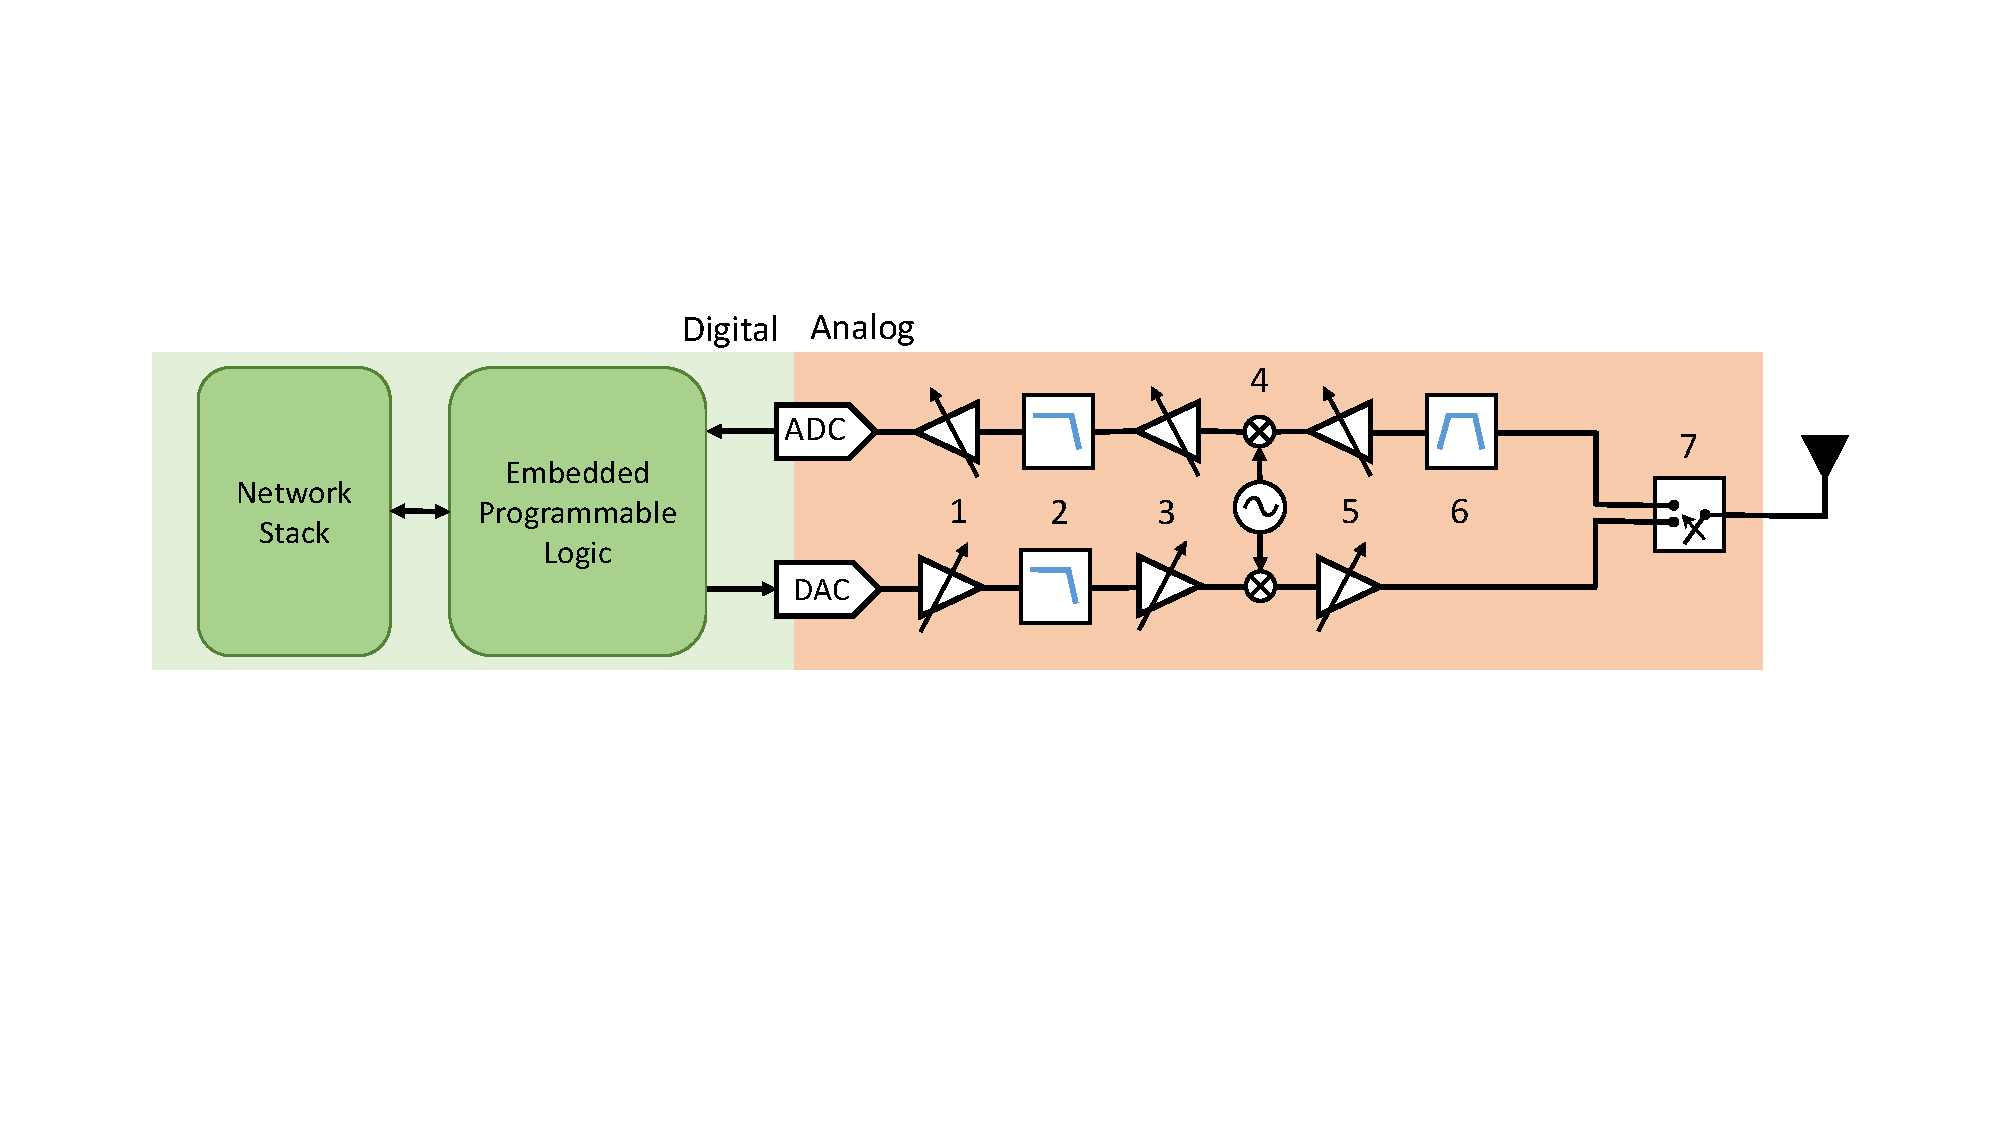
\includegraphics[width=1\linewidth]{./figs/agc/generic_sdr}
\caption{Block diagram of a generalized Software-Defined Radio system.}
\label{fig_sdr_ideal}
\end{figure}

We present a generalized block diagram model of a single-radio \ac{SDR} in Figure~\ref{fig_sdr_ideal}.
While implementations of \acp{SDR} vary, our model captures key components (from left to right) considered in this work and generalizes well to most commercial \ac{SDR} architectures:
\begin{itemize}
	\item \textbf{Network stack} - signal processing components with non time-critical functions; for example: user scheduling, priority queuing, or layer-2 routing.
	\item \textbf{Programmable logic} - signal processing components with time-critical or hardware-accelerated functions, specifically for networks layers 1 and 2; for example: gain control, digital pre-distortion, forward error correction.
	\item \textbf{Analog/Digital interface} - \acp{ADC} and \acp{DAC} provide the interface between digital and analog domains by converting digital samples to analog voltages and vice-versa.
	\item \textbf{Analog Gain Block (1)} - controls the amplitude of the signal entering or leaving the ADC/DAC.
	\item \textbf{Anti-aliasing filter (2)} - provides a low-pass filtering function on the analog signal to limit its information bandwidth to below the Nyquist sampling rate of the digital conversion step in order to avoid aliasing.
	\item \textbf{Analog Gain Block (3)} - controls the amplitude of the signal entering or leaving the analog mixer.
	\item \textbf{Frequency Up/Downconversion Mixing (4)} - a local center frequency, or \textit{carrier}, is multiplied by the analog signal to either up-convert or down-convert the signal to/from the RF frequency.
	\item \textbf{RF Gain Block (5)} - the input and output RF signal is amplified in order to meet the linearity or power budget requirements of the system's components.
	\item \textbf{Receive Band-Pass Filter (6)} - a band-pass filter limits the frequency content of the signal input to the receive radio chain in order to limit noise ingress and harmonic interference from strong out-of-band signals.
	\item \textbf{Transmit/Receive Switch (7)} - shares a signal antenna with the transmit and receive circuits; while this work generally considers \ac{TDD} protocols, this system component can be replaced with a frequency duplexer to support \ac{FDD} protocols, as well.
\end{itemize}

	This is by no means an exhaustive enumeration of the signal conditioning components present in all \ac{SDR} systems, but captures the important features needed for the techniques and systems in this work while being generic enough to apply across a wide range of commercial \ac{SDR} platforms.

	In addition, the division of functions between ``programmable logic'' and ``network stack'' blocks is a soft delineation made for ease of discussion.
	For the purpose of this work, we consider programmable logic to be an \ac{FPGA} or similar digital logic, whereas the network stack is implemented in embedded C or higher layer computer languages on a general-purpose processor.
	This division matches well-known experimental \ac{SDR} platforms like those mentioned in Section~\ref{sec_related_sdr}.

\subsection{Direct Sampling RF}
	As digital circuit integration and speed increases, a new \ac{SDR} paradigm is emerging in recent years that further reduces the amount of analog components necessary, shifting the dividing line between digital and analog domains in Figure~\ref{fig_sdr_ideal} nearly all the way to the antenna.
	``Direct sampling RF'' systems first used a combination of filtering and aliased sampling to directly sample RF signals without a down-conversion mixing step \cite{psiaki2005design}.
	More recently, increases in the integration and speed of digital circuits now permit direct sampling \acp{ADC} at RF frequencies without the drawback of aliased sampling \cite{xilinx2017rfsoc}.
	Although widespread use of direct sampling architectures will obviate the need for some of the analog components discussed in this thesis, key contributions of \ac{AGC}, environmental \ac{MU-MIMO} studies, and our protocol design remain unchanged.

%#######################################################
\section{Two Port Scattering Parameters}
\label{sec_scattering}

	In order to present some of our circuit design techniques, it will be necessary to be familiar with the definition and notation of normalized scattering, or S-parameters.
	The following discussion is a summary of the discussion and derivation by Yarman \cite{yarman2010design} and Orfanidis \cite{orfanidis2002electromagnetic} to describe a lossless two-port device.
	
\begin{figure}[h]
\centering
  \includegraphics[width=0.4\linewidth]{figs/matching/general_2_port}   
    \caption{General diagram of a lossless linear 2-port device with scattering parameters.}
\label{fig_general_2_port}
\end{figure}
	
	Consider Figure~\ref{fig_general_2_port}, a linear two-port microwave device that is excited by a complex source or ``generator'' impedance $Z_G$ and terminated in a complex load impedance $Z_L$.
	Assuming it it lossless, it is possible to describe the two-port system by describing the relationship of any incident and reflected voltage wave characterized by the wave variables $a_i, b_i$, where the current is defined in the direction of the corresponding $a_i$ vector and the characteristic reference impedance of the system is $Z_0$.
\begin{align}
a_1 &= \frac{V_1+Z_0 I_1}{2\sqrt{Z_0}}  &a_2 = \frac{V_2+Z_0 I_2}{2\sqrt{Z_0}} \\
b_1 &= \frac{V_1-Z_0 I_1}{2\sqrt{Z_0}}  &b_2 = \frac{V_2-Z_0 I_2}{2\sqrt{Z_0}}
\end{align}
This results in a relationship between incident and reflected traveling waves:
\begin{align}
	b_1 &= S_{11}a_1 + S_{12}a_2 \\
	b_2 &= S_{21}a_1 + S_{22}a_2.
\end{align}
	The system of traveling wave equations forms a scattering matrix, $\mathbf{S}\in\mathbb{C}^{2\times2}$ for a two-port device, $\mathbf{S}\in\mathbb{C}^{4\times4}$ for a four-port device, etc, that completely characterizes the device's linear, lossless behavior.
	
	There are two important assumptions related to the use of S-parameters; the first is that each set of empirical S-parameter is measured within a system with arbitrary characteristic impedance $Z_0$.
	As a matter of convention, nearly all S-parameters are measured in reference to 50~$\Omega$ and we will assume that in the rest of this thesis.
	
	Second, S-parameters only capture \emph{linear} steady-state device behavior, and for this reason they are generally described as ``small-signal'' parameters. For example, as the input signal power to a two-port amplifier is increased close to the IP1dB point, or the point where the amplifier becomes saturated and the output power decreases by 1~dB from ideal, non-linear behavior will be observed, requiring ``large-signal'' design techniques like load-pull analysis.
	Quaglia and Cripps present an excellent discussion of recent developments and models for power amplifiers operating in the saturated regime \cite{quaglia2017reappraisal}.
	We instead focus on linear operating conditions and small-signal designs for our system in order to preserve the simplicity of each radio chain within a complex many-antenna system, leaving energy efficiency optimization to future work.

For the system in Figure~\ref{fig_general_2_port}, it is also useful to define generator and load \emph{reflection coefficients} that describe the portion of a reflected incident wave with characteristic reference impedance $Z_0$ into a load.
\begin{equation}
\Gamma_G = \frac{Z_G - Z_0}{Z_G + Z_0},~~~ \Gamma_L = \frac{Z_L - Z_0}{Z_L + Z_0}
\end{equation}

	In this work, we will use the $\hat{(\cdot)}$ notation to indicate a reflection coefficient that is cascaded into a non-reference impedance.
	For example, $\hat{S}_{11}$ in Figure~\ref{fig_general_2_port} is the reflection coefficient of the active two-port terminated in an arbitrary load impedance $Z_L$ and can be written:
\begin{equation} \label{eq_}
\hat{S}_{11}=S_{11}+\frac{S_{12}S_{21}\Gamma_L}{1-S_{22}\Gamma_L},
\end{equation}
where in the case of $Z_L = Z_0 = 50~\Omega$, we see that this reduces to $\hat{S}_{11} = S_{11}$.
	Similarly, we can see that:
\begin{equation}
\hat{S}_{22}=S_{22}+\frac{S_{21}S_{12}\Gamma_G}{1-S_{11}\Gamma_G}.
\end{equation}

	We now have the tools needed to address the broadband power transfer network design problems presented in Section~\ref{sec_wurc_pa_design}.
	